\section{Experiment 10G: vehicle-class control-relevance gate}
\label{sec:experiment10g}

\paragraph{Purpose and precondition.}
Experiment 10F established a statistically repeatable but practically modest
control benefit of FederatedLearned over Global. Experiment 10G tests a
proposed route to a stronger effect: introduce physically interpretable
vehicle classes and steering-actuator dynamics. This experiment is an oracle
prerequisite gate, not an FL comparison. Learned clustering and finite-data
estimation are intentionally excluded. A federated extension is justified
only if known vehicle classes first provide a meaningful control advantage
over a single pooled model.

\paragraph{Extended nonlinear plant.}
The tanh-tire bicycle plant is augmented by the applied steering angle
$\delta_a$,
\begin{equation}
 x=[\beta,r,\delta_a]^\top,\qquad
 \dot{\delta}_a=\frac{\delta_{\mathrm{cmd}}-\delta_a}{\tau_\delta}.
\end{equation}
The compact, SUV, and sport centers in Table~\ref{tab:experiment10g-fleet}
vary mass, yaw inertia, geometry, axle cornering stiffness, and actuator time
constant. Each confirmation fleet contains ten clients per class. Independent
bounded scatter is $\pm5\%$ in mass, $\pm7\%$ in inertia, $\pm2\%$ in geometry,
$\pm8\%$ in stiffness, and $\pm15\%$ in $\tau_\delta$.

\begin{table}[htbp]
\centering
\caption{Experiment 10G vehicle-class centers. Stiffnesses are in kN/rad.}
\label{tab:experiment10g-fleet}
\begin{tabular}{lrrrrrrr}
\toprule
Class & $m$ & $I_z$ & $l_f$ & $l_r$ & $C_f$ & $C_r$ & $\tau_\delta$\\
 & kg & kg m$^2$ & m & m & & & s\\
\midrule
Compact & 1300 & 1900 & 1.10 & 1.50 & 70 & 75 & 0.10\\
SUV     & 2100 & 3900 & 1.35 & 1.70 & 90 & 100 & 0.18\\
Sport   & 1550 & 2350 & 1.25 & 1.45 & 105 & 115 & 0.07\\
\bottomrule
\end{tabular}
\end{table}

\paragraph{Oracle models and controller protocol.}
At each of eleven speeds from 10 to 30~m/s, the exact discrete Jacobian of the
three-state plant is computed. Global averages the matrices of all 30 clients,
OracleClass averages within the known class, and ClientExact retains each
client's matrices. All three use the same scheduled four-state LQI structure,
including yaw-error integration. Six weight candidates are evaluated on five
development fleets using ClientExact only. The selected candidate is
\begin{equation}
 Q=\operatorname{diag}(100,100,10,2000),\qquad R=0.1.
\end{equation}
It minimizes development mean tracking among candidates with all trajectories
feasible and less than 5\% mean saturation. Architecture comparison then uses
ten untouched fleets, seeds 441--450, and the frozen moderate and hard 10F
maneuvers. The proposed gate requires at least 5\% Global degradation relative
to ClientExact, at least 40\% recovery of that gap by OracleClass, a positive
paired confidence interval, and complete class-controller feasibility.

\begin{table}[htbp]
\centering
\caption{Experiment 10G confirmation yaw-rate RMSE in deg/s, averaged over ten fleets.}
\label{tab:experiment10g-summary}
\begin{tabular}{llrrr}
\toprule
Maneuver & Method & Mean client & Worst client & Mean saturation\\
\midrule
Moderate & Global       & 0.10281 & 0.14903 & 0.000\\
Moderate & OracleClass  & 0.10471 & 0.14996 & 0.000\\
Moderate & ClientExact  & 0.10294 & 0.13688 & 0.000\\
\midrule
Hard & Global           & 0.36339 & 0.65306 & 0.0169\\
Hard & OracleClass      & 0.38063 & 0.67296 & 0.0197\\
Hard & ClientExact      & 0.42267 & 2.05197 & 0.0246\\
\bottomrule
\end{tabular}
\end{table}

\begin{figure}[htbp]
\centering
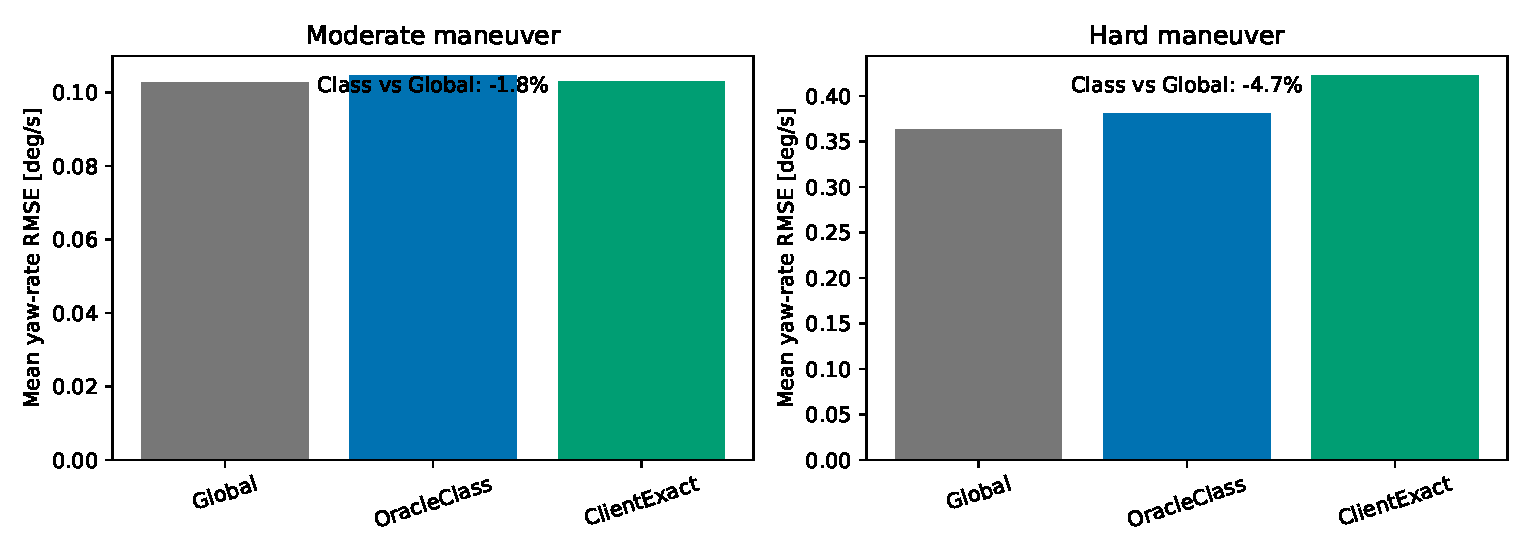
\includegraphics[width=0.92\linewidth]{../results/figures/experiment_10g_vehicle_class_gate.pdf}
\caption{Experiment 10G oracle architecture comparison. Known vehicle classes
do not improve mean nonlinear closed-loop tracking over the pooled controller.}
\label{fig:experiment10g}
\end{figure}

\paragraph{Result.}
The gate fails. OracleClass is 1.85\% worse than Global in moderate mean
tracking and 4.74\% worse in hard mean tracking. The paired 95\% intervals are
$[-2.15,-1.56]\%$ and $[-5.09,-4.39]\%$, respectively, where positive would
favor OracleClass. OracleClass loses to Global on mean tracking in every
confirmation fleet. All trajectories remain within the sideslip feasibility
limit, so the result is not caused by numerical divergence.

ClientExact also does not establish the assumed oracle advantage. In the hard
maneuver, three SUV clients enter sustained command saturation and increase
the fleet-level worst-client result. Their exact nominal LQI controllers are
more aggressive near the nonlinear tire and actuator constraints, whereas
matrix averaging produces a more conservative Global controller. A disclosed
post-hoc diagnostic replaces the selected controller by the adjacent, more
conservative development-approved candidate
$Q=\operatorname{diag}(50,75,5,1500)$, $R=0.15$. It removes the extreme SUV
outliers, but Global still has lower mean error than both OracleClass and
ClientExact in both maneuvers. Thus the conclusion is not rescued by a small
change in LQI weights.

\paragraph{Interpretation and decision.}
Adding vehicle classes and a first-order steering actuator does not by itself
create a stronger knowledge-sharing argument. The present LQI design is robust
to the structured plant variation, while nominal specialization can reduce
robustness under nonlinear constraints. Increasing parameter ranges or tuning
against the opened confirmation fleets would manufacture a gap rather than
establish one. We therefore stop this branch before adding FL.

The next defensible route is to change the control question rather than merely
the fleet: use a constraint-aware or robust synthesis objective, or quantify
the amount of local excitation needed to certify a controller over unseen
operating regions. Such a study must first show an oracle advantage on new
development data and reserve another untouched confirmation set.

\paragraph{Reproducibility.}
The configuration and implementation are in
\path{code/config/experiment_10g.json} and
\path{code/experiments/experiment_10g_vehicle_class_gate.py}. Controller
selection, client-level confirmation data, summaries, comparisons, gate
decisions, the figure, and provenance hashes are stored under
\path{results}.
